\documentclass{standalone}
\usepackage{pgfplots, tikz}
\pgfplotsset{compat=1.18}

\begin{document}

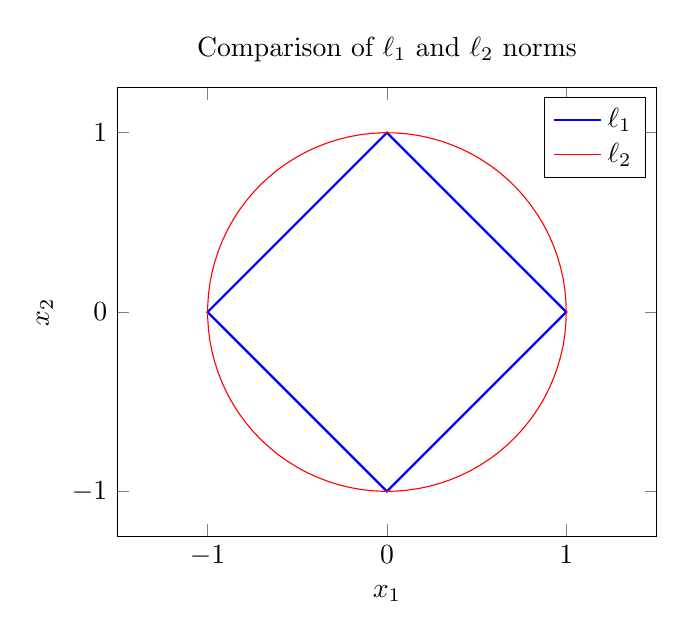
\begin{tikzpicture}
  \begin{axis}[
      axis lines = box,
      axis equal,
      xlabel = {$x_1$},
      ylabel = {$x_2$},
      xmin = -1, xmax = 1,
      ymin = -1.25, ymax = 1.25,
      xtick={-1, 0, 1},
      ytick={-1, 0, 1},
      grid = none,
      title = {Comparison of $\ell_1$ and $\ell_2$ norms},
      legend entries = {$\ell_1$, $\ell_2$},
    ]

    % l1 norm - square
    \addplot[thick, blue] coordinates {(0,-1) (1,0) (0,1) (-1,0)} -- cycle;
    % l2 norm - circle
    \addplot[
      domain=0:360,
      samples=100,
      color=red
    ] ({cos(x)}, {sin(x)});

  \end{axis}
\end{tikzpicture}

\end{document}
